\documentclass[11pt]{article}

% ======================================================================
%  Page geometry
% ======================================================================
\usepackage[a4paper,margin=1.1in]{geometry}

% ======================================================================
%  Math  (load AMS packages before the math font to avoid \Bbbk clash)
% ======================================================================
\usepackage{amsmath,amssymb,amsthm}
\usepackage{mathtools}

% ======================================================================
%  Fonts & typography  (Palatino-style text + matching math)
% ======================================================================
\usepackage[T1]{fontenc}
\usepackage{newpxtext}
\let\Bbbk\relax            % newpxmath redefines \Bbbk; avoid the clash
\usepackage{newpxmath}
\usepackage{bm}
\usepackage{microtype}

% ======================================================================
%  Tables, lists, colour, boxes, links, headings
% ======================================================================
\usepackage{booktabs}
\usepackage{enumitem}
\usepackage{graphicx}
\graphicspath{{figures/}}
\usepackage{xcolor}
\usepackage[most]{tcolorbox}
\usepackage{titlesec}
\usepackage[colorlinks=true]{hyperref}

\definecolor{accent}{HTML}{1F4E79}   % deep blue
\definecolor{accentlt}{HTML}{2E74B5} % lighter blue
\definecolor{boxbg}{HTML}{F2F6FB}    % pale blue box fill

\hypersetup{
  linkcolor=accent,
  citecolor=accent,
  urlcolor=accentlt,
}

% --- Coloured section headings ---
\titleformat{\section}
  {\normalfont\Large\bfseries\color{accent}}{\thesection}{0.7em}{}
\titleformat{\subsection}
  {\normalfont\large\bfseries\color{accentlt}}{\thesubsection}{0.6em}{}

% --- Paragraph style: open, unindented ---
\setlength{\parindent}{0pt}
\setlength{\parskip}{0.55em}

% --- Highlighted "key result" box for the central equations ---
\newtcolorbox{keybox}[1][]{
  enhanced, breakable,
  colback=boxbg, colframe=accent,
  boxrule=0.6pt, arc=3pt,
  left=10pt, right=10pt, top=8pt, bottom=8pt,
  fonttitle=\bfseries, coltitle=white,
  attach boxed title to top left={yshift=-2mm, xshift=4mm},
  boxed title style={colback=accent, arc=2pt},
  #1
}

% ======================================================================
%  Notation macros
% ======================================================================
\newcommand{\Znn}{\mathbb{Z}_{\geq 0}}            % non-negative integers
\newcommand{\Reals}{\mathbb{R}}
\newcommand{\Zsp}{\mathcal{Z}}                    % joint state space
\newcommand{\Ssp}{\mathcal{S}}                    % anatomical sites
\newcommand{\Csp}{\mathcal{C}}                    % clonotype set
\newcommand{\Rsp}{\mathcal{R}}                    % forward steps (source timepoints)
\newcommand{\Dsp}{\mathcal{D}}                    % data
\newcommand{\simplex}[1]{\Delta^{#1}}
\newcommand{\Nsrc}{N^{\mathrm{src}}}
\newcommand{\Ndst}{N^{\mathrm{dst}}}              % retained for the (deferred) plate figure
\newcommand{\dsrc}{d^{\mathrm{src}}}
\newcommand{\E}{\mathbb{E}}
\newcommand{\vq}{\mathfrak{q}}                    % variational distribution
\DeclareMathOperator{\Cat}{Categorical}
\DeclareMathOperator{\Mult}{Multinomial}
\DeclareMathOperator{\Dir}{Dirichlet}
\DeclareMathOperator{\Pois}{Poisson}
\DeclareMathOperator{\Gam}{Gamma}

\theoremstyle{definition}
\newtheorem*{remark}{Remark}

% ======================================================================
%  Title
% ======================================================================
\title{\bfseries\color{accent}\Large A Bayesian Population-Dynamics Model for
Clonal T Cells\\[2pt] across Tissue and Phenotype in Glioblastoma}
\date{\today}

\begin{document}
\maketitle

{\small\tableofcontents}
\vspace{1em}

% ======================================================================
\section{Setup}
% ======================================================================

We observe annotated T cells from multiple patients, anatomical sites, and
study timepoints. Each observed cell carries five labels: a patient, a TCR
clonotype, a study timepoint, an anatomical site, and a discrete T-cell
phenotype state.

The data are represented as aggregate
clone-by-timepoint-by-site-by-phenotype counts, from which we construct
clone-level observations across forward study steps.

\subsection{Indices}

We use the following indices throughout.
\begin{itemize}[leftmargin=1.4em, itemsep=2pt]
  \item Patients: $i = 1,\ldots,I$.
  \item TCR clonotypes within patient $i$: $c = 1,\ldots,C_i$.
  \item Shared study timepoints: $r \in \{1,\ldots,R\}$, ordered as
        $\tau_1 < \tau_2 < \cdots < \tau_R$. The timepoint labels are
        comparable across patients.
  \item Anatomical site: $s \in \Ssp$, with
        $\Ssp = \{\mathrm{PBMC},\, \mathrm{CSF},\, \mathrm{Tumor}\}$.
  \item Annotated T-cell phenotype state: $k \in \{1,\ldots,K\}$. In the
        current application $K = 11$, and all phenotypes share a single
        phenotype space.
\end{itemize}

\subsection{Observed count tensor}

For each patient $i$, clonotype $c$, timepoint $r$, site $s$, and phenotype
$k$, let
\[
  Y_{icrsk} \in \Znn
\]
be the observed number of cells assigned to that combination: how many cells
from patient $i$, clonotype $c$, and timepoint $r$ were sampled from site $s$
and assigned phenotype $k$. Collecting the site and phenotype axes,
\[
  Y_{icr} \in \Znn^{\,|\Ssp| \times K}
\]
is the tissue-by-phenotype count tensor for clonotype $c$ in patient $i$ at
timepoint $r$.

Each tissue sample also carries a sequencing depth and a missingness flag. For
patient $i$, timepoint $r$, and tissue $s$, let
\[
  d_{i,r,s} \in \Znn
\]
be the per-sample sequencing depth: the VDJ cell count for the Cell~Ranger run
of that $(\text{patient},\text{timepoint},\text{tissue})$ sample. It is the
Poisson exposure used below. Let
\[
  m_{i,r,s} \in \{0,1\}
\]
be the missingness indicator, equal to $1$ when that sample was profiled and
$0$ otherwise.

\subsection{Joint tissue--phenotype state space}

The model operates on the joint tissue--phenotype state space
\[
  \Zsp = \Ssp \times \{1,\ldots,K\},
  \qquad
  z = (s,k),
\]
where $s$ is the tissue and $k$ is the phenotype. Since $|\Ssp| = 3$ and
$K = 11$, the number of joint states is
\[
  L \;=\; |\Zsp| \;=\; |\Ssp|\,K \;=\; 33 .
\]
The model therefore tracks clone counts across a $33$-state
tissue--phenotype space. When describing transitions we write the source state
as $z = (a,u)$ and the destination state as $z' = (b,v)$, where $a,b \in \Ssp$
are source and destination tissues and $u,v \in \{1,\ldots,K\}$ are source and
destination phenotypes.

\subsection{Valid forward steps}

Forward steps are defined per patient. For patient $i$, let
$\Rsp_i \subseteq \{1,\ldots,R-1\}$ be the set of source timepoints at which
patient $i$ has a valid forward step. We index a step by its source timepoint
$r \in \Rsp_i$; the step runs from timepoint $r$ to the next sampled timepoint,
written $r+1$. Thus $r$ is not a matrix index---it simply labels a forward step
within patient $i$ by where it starts.

\begin{remark}[Skipped timepoints]
Writing the destination as $r+1$ assumes consecutive sampling. When a patient is
missing a timepoint---so that, say, $T_1$ and $T_3$ are paired---$r+1$ should be
read as the \emph{next available} timepoint for that patient. Which timepoints
are paired is a data-preprocessing detail and does not change anything below.
\end{remark}

Each $r \in \Rsp_i$ is one observed forward step. Steps such as
$T_1 \!\to\! T_2$, $T_2 \!\to\! T_3$, and $T_3 \!\to\! T_4$ are treated as
repeated observations of the \emph{same} forward process: the growth matrix is
shared across all patients and steps, and the indices $i$ and $r$ merely
organize observations rather than selecting a separate matrix.

\subsection{Clone-level observations within a step}

Fix a patient $i$, a valid step $r \in \Rsp_i$, and a clonotype $c$ observed for
that patient. The source and destination count vectors over the joint state
space are read directly off the count tensor at timepoints $r$ and $r+1$,
\[
  x_{irc}(s,k) = Y_{i\, c\, r\, s\, k},
  \qquad
  y_{irc}(s,k) = Y_{i\, c\, (r+1)\, s\, k},
  \qquad (s,k)\in\Zsp,
\]
so $x_{irc} \in \Znn^{L}$ and $y_{irc} \in \Znn^{L}$.

The source enters the model only after dividing out the source sequencing
depth. The \emph{depth-rescaled source} is
\[
  \tilde{x}_{irc}(z) = \frac{x_{irc}(z)}{\dsrc_{ir,s}},
  \qquad s = \mathrm{tissue}(z),
  \qquad \dsrc_{ir,s} = d_{i,r,s},
\]
i.e.\ each source count is divided by the source-timepoint depth of its tissue.
It is treated as a fixed, known plug-in, not a random quantity: source abundance
enters after dividing out source depth, and residual source-sampling variation
is not modeled.

We retain clonotypes present at the \emph{source} end of the step,
\[
  \Csp_{ir}
  =
  \bigl\{\,
    c \in \{1,\ldots,C_{i}\}
    \;:\;
    \Nsrc_{irc} > 0
  \,\bigr\},
  \qquad
  \Nsrc_{irc} = \sum_{z\in\Zsp} x_{irc}(z) .
\]
A destination total of zero is now a modeled observation---a contraction or
death signal---not an exclusion criterion. This gives the data hierarchy
\[
  i
  \;\longrightarrow\;
  r \in \Rsp_i
  \;\longrightarrow\;
  c \in \Csp_{ir},
\]
patients contain valid forward steps, and each forward step has a retained set
of source-present clonotypes. A \emph{clone-level forward observation} is the
triple $(i,r,c)$; for compact notation we write
\[
  j \;\equiv\; (i,r,c),
  \qquad
  x_j = x_{irc},
  \qquad
  \tilde{x}_j = \tilde{x}_{irc},
  \qquad
  y_j = y_{irc} .
\]

The destination vector $y_j$ keeps its per-tissue structure: each tissue
sub-block $\{(s',k) : k = 1,\ldots,K\}$ of $y_j$ carries its own destination
depth $d_{j,s'} = d_{i,\,r+1,\,s'}$ and missingness flag
$m_{j,s'} = m_{i,\,r+1,\,s'}$.

\subsection{Two kinds of destination zero}

Destination zeros are part of the likelihood specification, and the two kinds
are treated differently.
\begin{enumerate}[leftmargin=2em, itemsep=3pt]
  \item \textbf{Missing sample} ($m_{j,s'} = 0$). The tissue sub-block
        $\{(s',k)\}$ was not profiled at the destination timepoint. It is
        excluded from the likelihood entirely---masked out, never entered as a
        zero count.
  \item \textbf{Depth-zero} ($m_{j,s'} = 1$, clone not captured). A genuine
        observed zero, modeled natively by the Poisson likelihood below: a small
        mean $d_{j,s'}\,\mu_j(z')$ emits zero with positive probability while
        $\mu_j(z') > 0$. No zero-inflation component is added.
\end{enumerate}
The depth-zero mechanism is what permits a clone to be absent at one step and
present at the next.

\subsection{Setup summary}

The setup produces the clone-level forward observations
\[
  \Dsp = \bigl\{ (\tilde{x}_j,\, y_j,\, d_j,\, m_j,\, i_j,\, r_j,\, c_j) \bigr\}_{j=1}^{J},
  \qquad j \equiv (i_j, r_j, c_j),
\]
each carrying a depth-rescaled source vector, a destination count vector, the
per-tissue destination depths $d_j = (d_{j,s'})_{s'\in\Ssp}$ and missingness
flags $m_j = (m_{j,s'})_{s'\in\Ssp}$, and a patient / step / clonotype identity.
The count vectors live in the joint tissue--phenotype state space
$\Zsp = \Ssp \times \{1,\ldots,K\}$, with $|\Zsp| = 33$.

\subsection{Notation summary}

Table~\ref{tab:notation} collects the core modeling symbols; the variational
quantities used only for fitting (the Gamma parameters
$\mathrm{shape}_{zz'},\mathrm{rate}_{zz'}$, the responsibilities $r_{jzz'}$, and
$\psi$) are introduced where they are used in the inference section.

\begin{table}[h]
\centering
\renewcommand{\arraystretch}{1.25}
\begin{tabular}{@{}ll@{}}
\toprule
\textbf{Symbol} & \textbf{Meaning}\\
\midrule
$i = 1,\ldots,I$              & patient index\\
$c = 1,\ldots,C_i$           & TCR clonotype within patient $i$\\
$r \in \{1,\ldots,R\}$       & shared study timepoint, $\tau_1<\cdots<\tau_R$\\
$s \in \Ssp$                 & anatomical site, $\Ssp=\{\mathrm{PBMC},\mathrm{CSF},\mathrm{Tumor}\}$\\
$k \in \{1,\ldots,K\}$       & phenotype state ($K=11$)\\
$z = (s,k) \in \Zsp$         & joint tissue--phenotype state ($L=|\Zsp|=33$)\\
$Y_{icrsk}$                  & observed count tensor\\
$d_{i,r,s}$                  & per-sample sequencing depth (Poisson exposure)\\
$m_{i,r,s} \in \{0,1\}$      & sample missingness indicator\\
$\Rsp_i$                     & valid forward steps for patient $i$ ($\subseteq\{1,\ldots,R-1\}$)\\
$r \in \Rsp_i$               & forward step, from source timepoint $r$ to $r+1$\\
$\Csp_{ir}$                  & clonotypes present at the source end of step $r$\\
$j = (i_j,r_j,c_j)$          & clone-level observation, $j=1,\ldots,J$\\
$x_j,\,y_j \in \Znn^{L}$     & source / destination count vectors\\
$\tilde{x}_j$                & depth-rescaled source, $\tilde{x}_j(z)=x_j(z)/\dsrc_{j,s}$\\
$M \in \Reals_{\geq 0}^{L\times L}$ & non-negative growth matrix (free row sums)\\
$\mu_j = \tilde{x}_j M \in \Reals_{\geq 0}^{L}$ & destination intensity vector\\
$a_z,\,b_z$                  & Gamma prior shape / rate for row $z$\\
$w_{jzz'}$                   & backward attribution probability\\
$\xi_{jzz'}$                 & latent allocation count (computational)\\
$\Dsp$                       & full dataset\\
\bottomrule
\end{tabular}
\caption{Core modeling notation.}
\label{tab:notation}
\end{table}

% ======================================================================
\section{Joint Tissue--Phenotype Growth Matrix}
% ======================================================================

The central latent object is a single joint tissue--phenotype \emph{growth
matrix}
\[
  M \in \Reals_{\geq 0}^{L\times L},
  \qquad L = 33,
\]
whose rows are source states and whose columns are destination states. For
source state $z = (a,u)$ and destination state $z' = (b,v)$, the entry $M_{zz'}$
is the expected number of destination-$z'$ cells produced per source-$z$ cell
over one forward step (one $8$-week interval):
\[
  M_{zz'} = M_{(a,u),(b,v)}
  =
  \E[\,\text{cells in state } (b,v) \text{ at } r+1
        \text{ per cell in state } (a,u) \text{ at } r\,] .
\]

\subsection{Non-negative rows and growth factors}

$M$ has non-negative entries, $M_{zz'} \geq 0$, and \emph{free} row sums---rows
are not constrained to sum to one. The row sum
\[
  g_z \;=\; \sum_{z'\in\Zsp} M_{zz'}
\]
is the net $8$-week growth factor of source state $z$: $g_z > 1$ is net
expansion of that state, $g_z < 1$ net contraction or death.

\subsection{Destination intensity vector}

For observation $j$ with depth-rescaled source $\tilde{x}_j$, the destination
\emph{intensity vector} is the pushforward of $\tilde{x}_j$ through $M$:

\begin{keybox}[title={Central growth calculation}]
\[
  \mu_j = \tilde{x}_j M \in \Reals_{\geq 0}^{L},
  \qquad\text{equivalently}\qquad
  \mu_j(z')
  =
  \sum_{z\in\Zsp} \tilde{x}_j(z)\, M_{zz'} .
\]
\end{keybox}

The expected destination count in state $z'$ scales the intensity by the
destination depth of its tissue,
\[
  \E\!\left[ y_j(z') \mid M \right] = d_{j,s'}\, \mu_j(z'),
  \qquad s' = \mathrm{tissue}(z') .
\]
There is no simplex constraint on $\mu_j$ and no conditioning on a destination
total.

\subsection{Role of forward steps}

The same matrix $M$ is used for every patient $i$ and step $r \in \Rsp_i$. The
pair $(i,r)$ selects which source and destination vectors to build, not a
different matrix; all steps are repeated observations of a common one-step
forward process.

% ======================================================================
\section{Bayesian Reading of the Growth Matrix}
% ======================================================================

The matrix $M$ is a latent non-negative kernel of per-cell destination
intensities over the joint tissue--phenotype state space.

\subsection{Forward generative reading}

Read forward, the model is a Poisson superposition. Treating the depth-rescaled
source as a population with $\tilde{x}_j(z)$ cells in each state $z$, each
source cell in state $z$ independently emits a Poisson-distributed number of
cells into each destination state $z'$ with mean $M_{zz'}$. Summing these
emissions over all source states and scaling by the destination depth, the
destination-$z'$ count is, by Poisson superposition,
\[
  y_j(z') \mid M
  \;\sim\;
  \Pois\!\Bigl( d_{j,s'} \sum_{z\in\Zsp} \tilde{x}_j(z)\, M_{zz'} \Bigr)
  =
  \Pois\!\bigl( d_{j,s'}\, \mu_j(z') \bigr) .
\]

\subsection{Likelihood for destination counts}

\begin{keybox}[title={Observation likelihood}]
\[
  y_j(z') \;\sim\; \Pois\!\bigl( d_{j,s'}\, (\tilde{x}_j M)(z') \bigr),
  \qquad s' = \mathrm{tissue}(z'),
\]
evaluated only over non-missing destination sub-blocks ($m_{j,s'} = 1$). The
latent matrix enters the likelihood only through the intensity
$\mu_j = \tilde{x}_j M$.
\end{keybox}

\subsection{Prior over growth-matrix entries}

Each entry receives an independent Gamma prior in shape--rate form,
\[
  M_{zz'} \;\sim\; \Gam(a_z, b_z),
\]
with row-specific shape $a_z$ and rate $b_z$.

\begin{remark}[Support restrictions are an implementation detail]
In practice the implementation may exclude biologically implausible transitions
by fixing the corresponding entries of $M$ to zero (placing the Gamma prior only
on the retained entries of each row). This sparsifies $M$ but does not change
the form of the model; sums over destination states below are read over the
retained entries. We treat the support as a fixed preprocessing choice.
\end{remark}

For the likelihood to support the data, the support guard is: for every
non-missing destination state $z'$ with $y_j(z') > 0$, at least one source state
in the support of $\tilde{x}_j$ must reach $z'$ (i.e.\ have $M_{zz'} > 0$).

\subsection{Posterior over growth matrices}

After observing the data $\Dsp$, inference targets the posterior
$p(M \mid \Dsp)$, which captures uncertainty about the joint tissue--phenotype
growth kernel after all clone-level forward observations. Posterior summaries
include posterior means $\E[M_{zz'} \mid \Dsp]$ and credible intervals for
individual entries.

\subsection{Posterior predictive destination counts}

Because $M$ is latent, the intensity $\mu_j = \tilde{x}_j M$ is also uncertain.
Posterior draws of $M$ induce replicated destination counts
\[
  y_j^{\mathrm{rep}}(z') \;\sim\; \Pois\!\bigl( d_{j,s'}\, \mu_j(z') \bigr)
\]
over the non-missing sub-blocks ($m_{j,s'} = 1$).

\subsection{Backward attribution}
\label{sec:backward}

The reverse question---which source state produced an observed destination
cell---is a posterior attribution. For observation $j$,
\[
  w_{jzz'}
  =
  \frac{\tilde{x}_j(z)\, M_{zz'}}
       {\sum_{\tilde z\in\Zsp} \tilde{x}_j(\tilde z)\, M_{\tilde z z'}}
  =
  \frac{\tilde{x}_j(z)\, M_{zz'}}{\mu_j(z')} ,
\]
the same form as the forward intensity with source and destination roles
reversed. Because the destination counts are Poisson, these probabilities also
induce a multinomial decomposition of each observed count $y_j(z')$ into latent
source-to-destination allocation counts. Those counts are used only for fitting,
so we introduce them together with the inference algorithm in
Section~\ref{sec:inference-comp}.

% ======================================================================
\section{Full Generative Story}
\label{sec:generative}
% ======================================================================

The full model is a model for the one-step expansion and redistribution of clone
mass across tissue--phenotype states. It can be summarized as follows.

\begin{keybox}[title={Generative model}]
\begin{enumerate}[leftmargin=2em, itemsep=4pt]
  \item \textbf{State space.} Define
        $\Zsp = \Ssp \times \{1,\ldots,K\}$ with $|\Zsp| = 33$. Each state
        $z = (s,k)$ pairs an anatomical tissue with an annotated T-cell
        phenotype.

  \item \textbf{Growth-matrix entries.} For each source state $z$ and
        destination state $z'$, draw independently
        \[
          M_{zz'} \sim \Gam\!\bigl( a_z, b_z \bigr) .
        \]
        Entry $M_{zz'}$ is the expected number of destination-$z'$ cells per
        source-$z$ cell over one forward step.

  \item \textbf{Source.} For each patient $i$, step $r\in\Rsp_i$, and retained
        clonotype $c\in\Csp_{ir}$, form the observation $j = (i,r,c)$ and the
        fixed depth-rescaled source $\tilde{x}_j$.

  \item \textbf{Intensity.} Push the source forward,
        $\mu_j = \tilde{x}_j M$.

  \item \textbf{Observation.} For each non-missing destination sub-block
        ($m_{j,s'} = 1$), draw the destination counts
        \[
          y_j(z') \;\sim\; \Pois\!\bigl( d_{j,s'}\, \mu_j(z') \bigr),
          \qquad s' = \mathrm{tissue}(z') .
        \]
\end{enumerate}
\end{keybox}

Putting the pieces together, the generative model is, compactly,
\[
  M_{zz'} \sim \Gam\!\bigl(a_z, b_z\bigr),
  \qquad
  \mu_j = \tilde{x}_j M,
  \qquad
  y_j(z') \sim \Pois\!\bigl(d_{j,s'}\, \mu_j(z')\bigr)
  \quad (m_{j,s'} = 1),
\]
with the corresponding dependency structure shown in
Figure~\ref{fig:plate}.

\begin{figure}[htbp]
  \centering
  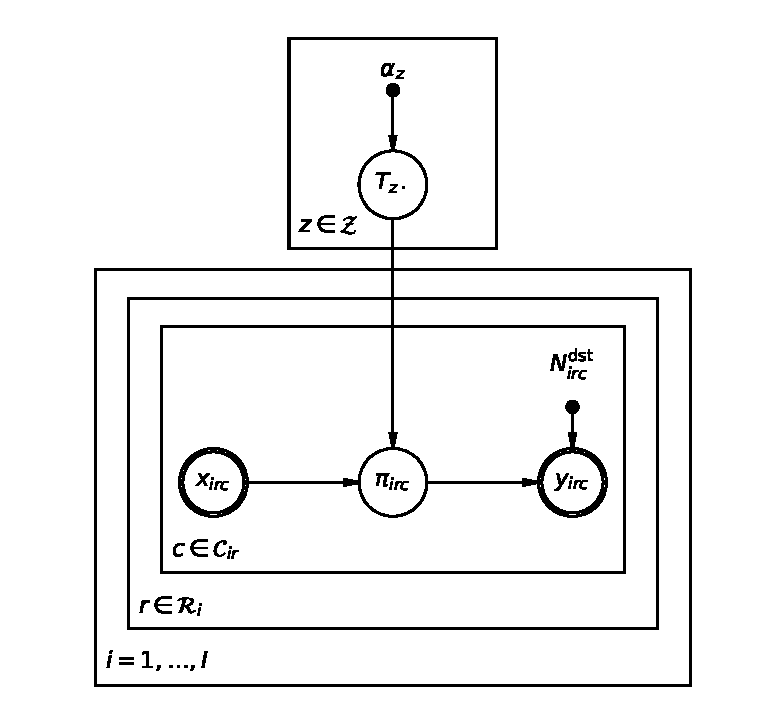
\includegraphics[width=0.78\linewidth]{plate_joint_transition.pdf}

  \smallskip
  {\small
  \begin{tabular}{@{}ll@{}}
    \toprule
    \textbf{Node} & \textbf{Meaning}\\
    \midrule
    $x_{irc}$ & observed source counts at the start of the step (over the $33$ states)\\
    $\tilde{x}_{irc}=x_{irc}/\dsrc_{irs}$ & depth-rescaled source (deterministic; folded into the $x\!\to\!\mu$ edge)\\
    $\mu_{irc}=\tilde{x}_{irc}M$ & destination intensity vector\\
    $y_{irc}$ & observed destination counts in tissue $s$ at the end of the step\\
    $M_{z\cdot}$ & latent growth-matrix row, shared across all patients and steps\\
    $d_{irs}$ & destination sequencing depth, Poisson exposure (fixed)\\
    $m_{irs}$ & sample missingness flag (fixed)\\
    $(a_z, b_z)$ & Gamma prior shape / rate (fixed)\\
    \bottomrule
  \end{tabular}}

  \caption{Plate diagram of the generative model (node key above). The rows
    $M_{z\cdot}$ are drawn once per source state $z$ from a Gamma prior
    $(a_z, b_z)$; this block sits \emph{outside} the patient plate, so a single
    $M$ is shared across all patients and steps. The observation side nests
    patient $i$, step $r\in\Rsp_i$, clone $c\in\Csp_{ir}$, and tissue
    $s\in\Ssp$. The depth-rescaled source $\tilde{x}_{irc}$ is pushed through
    $M$ to the intensity $\mu_{irc}=\tilde{x}_{irc}M$, and within each tissue
    sub-block the destination counts $y_{irc}$ are a Poisson draw with mean
    $d_{irs}\,\mu_{irc}$, gated by missingness $m_{irs}$. Double circles
    ($x_{irc}$, $y_{irc}$) mark observed quantities; solid dots
    ($(a_z, b_z)$, $d_{irs}$, $m_{irs}$) mark fixed inputs; the depth-rescaling
    $\tilde{x}_{irc}=\mathrm{Rescale}(x_{irc})$ is folded into the
    $x\!\to\!\mu$ edge. Latent allocation counts used for fitting are a
    computational augmentation introduced in Section~\ref{sec:inference-comp}.}
  \label{fig:plate}
\end{figure}

% ======================================================================
\section{Inference}
\label{sec:inference-comp}
% ======================================================================

Inference estimates the posterior over the shared growth matrix $M$. The
observed data are the clone-level forward observations $\Dsp$; the depth-rescaled
sources $\tilde{x}_j$, the depths $d_{j,s'}$, and the missingness flags
$m_{j,s'}$ are fixed inputs, as are the Gamma prior parameters $a_z, b_z$.

\subsection{Learned quantity}

The main learned object is the posterior $p(M \mid \Dsp)$. A single-entry
summary is
\[
  \E\!\left[ M_{(a,u),(b,v)} \mid \Dsp \right],
\]
the posterior mean number of destination-$(b,v)$ cells produced per
source-$(a,u)$ cell over one forward step.

\subsection{Variational approximation}

We approximate $p(M \mid \Dsp)$ by mean-field variational inference. The
difficulty is that an observed destination count in state $z'$ is a
\emph{superposition} of contributions from every source state $z$, and these
source-to-destination allocations are unobserved. Variational inference augments
the model with latent allocation counts and fits a factorized approximation by
coordinate ascent.

\subsection{Latent allocation counts}

Let $\xi_{jzz'}$ be the unobserved number of destination-$z'$ cells in
observation $j$ contributed by source state $z$. By Poisson superposition each
source contribution is itself Poisson,
$\xi_{jzz'} \sim \Pois\!\bigl( d_{j,s'}\, \tilde{x}_j(z)\, M_{zz'} \bigr)$
independently, and they decompose each observed destination count,
\[
  \sum_{z\in\Zsp} \xi_{jzz'} = y_j(z') .
\]
Conditional on the total $y_j(z')$, the allocations are multinomial with
probabilities equal to the backward attribution $w_{jzz'}$ of
Section~\ref{sec:backward}; variational inference replaces these with an
approximate responsibility $r_{jzz'}$.

\subsection{Variational family}

We adopt a mean-field factorization $\vq(M,\xi) = \vq(M)\,\vq(\xi)$. The growth
matrix receives independent Gamma factors, one per entry,
\[
  \vq(M)
  =
  \prod_{z\in\Zsp}\prod_{z'\in\Zsp}
    \Gam\!\bigl( M_{zz'};\, \mathrm{shape}_{zz'},\, \mathrm{rate}_{zz'} \bigr),
\]
and the allocation variables receive multinomial factors (a Poisson vector
conditioned on its total),
\[
  \vq(\xi)
  =
  \prod_{j=1}^{J} \prod_{z'\,:\,m_{j,s'}=1}
    \Mult\!\bigl( \xi_{j\cdot z'};\, y_j(z'),\, r_{j\cdot z'} \bigr),
\]
where $r_{jzz'}$ is the variational responsibility assigning destination state
$z'$ in observation $j$ to source state $z$.

\subsection{Coordinate updates}

The algorithm alternates between updating the allocation responsibilities
$r_{jzz'}$ and the Gamma parameters $(\mathrm{shape}_{zz'}, \mathrm{rate}_{zz'})$.

\subsubsection{Allocation update}

For each observation $j$, destination state $z'$ with $m_{j,s'}=1$, and source
state $z$,
\[
  r_{jzz'} \propto \tilde{x}_j(z)\,
  \exp\!\bigl( \E_{\vq}[\log M_{zz'}] \bigr),
\]
normalized over source states so that $\sum_{z\in\Zsp} r_{jzz'} = 1$ for each
$j$ and $z'$ (the common depth $d_{j,s'}$ cancels in the normalization). Under
the Gamma factor, the required expectation is
\[
  \E_{\vq}[\log M_{zz'}]
  =
  \psi(\mathrm{shape}_{zz'}) - \log(\mathrm{rate}_{zz'}),
\]
where $\psi$ is the digamma function.

\subsubsection{Entry update}

For each source state $z$ and destination state $z'$, the Gamma--Poisson
conjugate update is
\[
  \mathrm{shape}_{zz'}
  =
  a_z + \sum_{j} y_j(z')\, r_{jzz'},
  \qquad
  \mathrm{rate}_{zz'}
  =
  b_z + \sum_{j} d_{j,s'}\, \tilde{x}_j(z),
\]
where both sums run over observations whose destination sub-block $s'$ is
non-missing ($m_{j,s'} = 1$). The shape accumulates the expected number of
$z\!\to\!z'$ cells allocated from the data; the rate accumulates the
depth-weighted source exposure.

\subsection{Optimization objective}

The coordinate updates maximize the evidence lower bound (ELBO)
\[
  \mathcal{L}(\vq)
  =
  \E_{\vq}\!\left[ \log p(M,\xi,\Dsp) \right]
  -
  \E_{\vq}\!\left[ \log \vq(M,\xi) \right],
\]
and the algorithm iterates between the allocation update and the entry update
until $\mathcal{L}(\vq)$ stabilizes.

\subsection{Estimated growth matrix}

After convergence, the fitted growth matrix is the variational posterior mean of
each Gamma factor,
\[
  \widehat{M}_{zz'} = \E_{\vq}[M_{zz'}]
  =
  \frac{\mathrm{shape}_{zz'}}{\mathrm{rate}_{zz'}} ,
\]
explicitly \emph{not} normalized across destinations $z'$. The matrix
$\widehat{M}$ is the estimated one-step growth matrix over the $33$-state
tissue--phenotype space.

\subsection{Algorithm summary}

\begin{keybox}[title={Variational algorithm (CAVI)}]
\begin{enumerate}[leftmargin=2em, itemsep=4pt]
  \item \textbf{Initialize} the variational Gamma parameters
        $(\mathrm{shape}, \mathrm{rate})$.
  \item \textbf{Repeat until the ELBO $\mathcal{L}(\vq)$ converges:}
    \begin{itemize}[leftmargin=1.4em, itemsep=2pt, topsep=2pt]
      \item update the allocation responsibilities
            $r_{jzz'} \propto \tilde{x}_j(z)\,\exp\!\bigl(\E_{\vq}[\log M_{zz'}]\bigr)$;
      \item update the entry parameters
            $\mathrm{shape}_{zz'} = a_z + \sum_{j} y_j(z')\, r_{jzz'}$,
            $\mathrm{rate}_{zz'} = b_z + \sum_{j} d_{j,s'}\, \tilde{x}_j(z)$.
    \end{itemize}
  \item \textbf{Return} the posterior mean
        $\widehat{M} = \E_{\vq}[M]$.
\end{enumerate}
\end{keybox}

% ======================================================================
\section{Posterior Summaries}
% ======================================================================

With the variational posterior fitted and $\widehat{M}$ in hand, the following
quantities are read off it.

\subsection{Trafficking and growth}

The fitted matrix $\widehat{M}$ admits two readings, on its off-diagonal tissue
blocks and on its row sums.

\emph{Trafficking.} For source state $z = (a,u)$ and a destination tissue
$b \neq a$, the off-diagonal block sum
\[
  \tau_{z\to b} = \sum_{v=1}^{K} \widehat{M}_{(a,u),(b,v)}
\]
is the expected number of progeny of a source-$z$ cell that land in tissue $b$
over the step; summing over destination tissues $b \neq a$ gives the total
out-of-tissue trafficking from state $z$.

\emph{Growth.} The full row sum (diagonal block included)
\[
  g_z = \sum_{z'\in\Zsp} \widehat{M}_{zz'}
\]
is the net per-cell progeny count of source state $z$ over the step.

Off-diagonal block sums measure trafficking; the row sum, with the diagonal
included, measures net growth.

\subsection{Rate decomposition}

To express the step as per-week rates, define the generator
\[
  B = \frac{1}{\Delta t}\,\log \widehat{M},
  \qquad \Delta t = 8 \text{ weeks},
\]
the matrix logarithm of $\widehat{M}$ divided by the step length. The
off-diagonal entries $B_{zz'} \geq 0$ ($z' \neq z$) are the per-week trafficking
rates between states, and the row sums of $B$ are the net per-capita growth
rates per week. As above, the off-diagonal entries carry trafficking and the row
sums carry growth.

\end{document}
